% Motivation model diagram Heckhausen and Rheinberg
% Author: Stefan Kottwitz
\documentclass[tikz,border=10pt]{standalone}
\usetikzlibrary{matrix,arrows.meta}
\usetikzlibrary{fit}
\tikzset{
  centered/.style = { align=center, anchor=center },
     empty/.style = { font=\sffamily\Large, centered, text width=2cm },
     arrow/.style = { very thick, color=gray, ->, >=Triangle},
     harrow/.style = { very thick, color=blue, ->, >=Triangle},
     high/.style = {color = blue}
}
\newcommand*{\com}{Commit}


\def\Size{20pt}
\tikzset{
  file/.pic={
    \draw (0,-0.6*\Size) -- (0,0.6*\Size) -- 
        (0.7*\Size,0.6*\Size) -- (0.7*\Size,0.2*\Size) -- (1*\Size,0.2*\Size) -- 
        (1*\Size,-0.6*\Size) -- cycle;
    \draw (0.7*\Size,0.6*\Size) -- (1*\Size,0.2*\Size);

    \foreach \y in {-0.4*\Size,-0.2*\Size,0}{
      \draw (0.2*\Size,\y) -- (0.8*\Size,\y);
    }
    \draw (0.2*\Size,0.2*\Size) -- (0.6*\Size,0.2*\Size);
    \draw (0.2*\Size,0.4*\Size) -- (0.6*\Size,0.4*\Size);
  }
}

\begin{document}

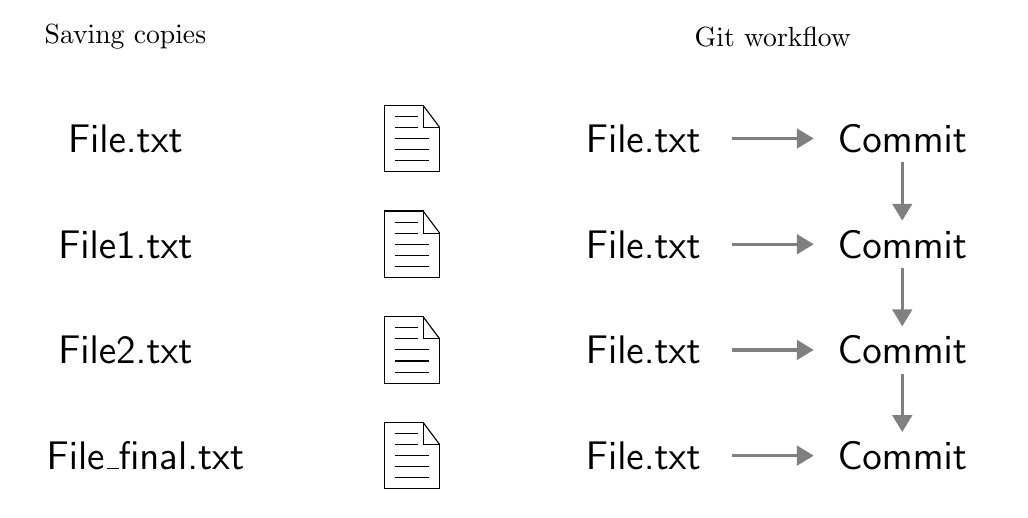
\begin{tikzpicture}
  \matrix (m)
    [
      matrix of nodes,
      nodes in empty cells,
      column sep      = 3em,
      row sep         = 5ex,
      column 1/.style = { nodes = { empty } },
      column 2/.style = { nodes = { empty } },
      column 3/.style = { nodes = { empty } },
      column 4/.style = { nodes = { empty } },
    ]
    {
        &  &  &  \\
        File.txt &  & File.txt & \com \\  % \textit{7f21c09}
        File1.txt &  & File.txt & \com \\ % \textit{d39ac60}
        File2.txt &  & File.txt & \com \\ % \textit{c78c64d}
        File\_final.txt &  & File.txt & \com \\ % \textit{cbdac1e}
    };
    \node[fit=(m-1-1)(m-1-1)]{Saving copies};
    \node[fit=(m-1-3)(m-1-4)]{Git workflow};
  \foreach \i/\j in {2/3,3/4,4/5} {
    \draw [arrow] (m-\i-4) -- (m-\j-4);
    \draw [arrow] (m-\i-3) -- (m-\i-4);
    \pic at (m-\i-2) {file};
  }
  \draw [arrow] (m-5-3) -- (m-5-4);
  \pic at (m-5-2) {file};
  
\end{tikzpicture}

\begin{tikzpicture}
  \matrix (m)
    [
      matrix of nodes,
      nodes in empty cells,
      column sep      = 3em,
      row sep         = 5ex,
      column 1/.style = { nodes = { empty } },
      column 2/.style = { nodes = { empty } },
      column 3/.style = { nodes = { empty } },
      column 4/.style = { nodes = { empty } },
    ]
    {
        &  &  &  \\
        File.txt &  & File.txt & \com \\  % \textit{7f21c09}
        &  & & \\ % \textit{d39ac60}
        &  & & \\ % \textit{c78c64d}
        &  & & \\ % \textit{cbdac1e}
    };
    \node[fit=(m-1-1)(m-1-1)]{Saving copies};
    \node[fit=(m-1-3)(m-1-4)]{Git workflow};
  \foreach \i/\j in {2/3} {
    \draw [arrow] (m-\i-4) -- (m-\j-4);
    % \draw [arrow] (m-\i-3) -- (m-\i-4);
    \pic at (m-\i-2) {file};
  }
  % \draw [arrow] (m-5-3) -- (m-5-4);
  % \pic at (m-5-2) {file};
  
\end{tikzpicture}

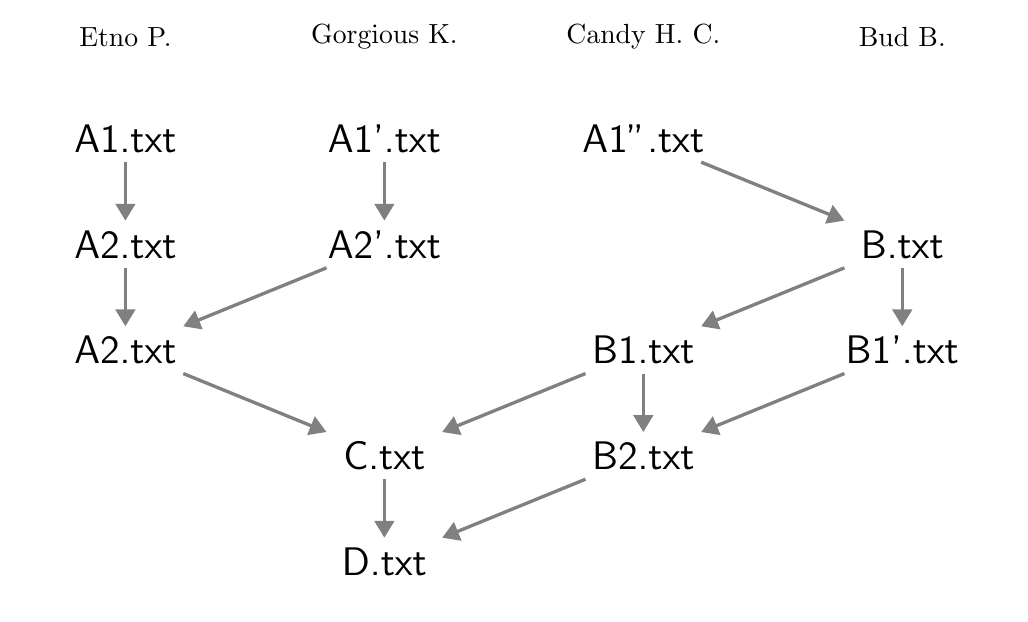
\begin{tikzpicture}
  \matrix (m)
    [
      matrix of nodes,
      nodes in empty cells,
      column sep      = 3em,
      row sep         = 5ex,
      column 1/.style = { nodes = { empty } },
      column 2/.style = { nodes = { empty } },
      column 3/.style = { nodes = { empty } },
      column 4/.style = { nodes = { empty } },
    ]
    {
        &  &  &  \\
        A1.txt & A1'.txt & A1''.txt &  \\ 
        A2.txt & A2'.txt &  & B.txt \\
        A2.txt &  & B1.txt & B1'.txt \\
        & C.txt & B2.txt &  \\
        & D.txt &  &  \\
    };
    \node[fit=(m-1-1)(m-1-1)]{Etno P.};
    \node[fit=(m-1-2)(m-1-2)]{Gorgious K.};
    \node[fit=(m-1-3)(m-1-3)]{Candy H. C.};
    \node[fit=(m-1-4)(m-1-4)]{Bud B.};
  
    \draw [arrow] (m-2-1) -- (m-3-1);
    \draw [arrow] (m-3-1) -- (m-4-1);
    \draw [arrow] (m-4-1) -- (m-5-2);

    \draw [arrow] (m-2-2) -- (m-3-2);
    \draw [arrow] (m-3-2) -- (m-4-1);
    \draw [arrow] (m-5-2) -- (m-6-2);

    \draw [arrow] (m-2-3) -- (m-3-4);
    \draw [arrow] (m-4-3) -- (m-5-3);
    \draw [arrow] (m-4-3) -- (m-5-2);
    \draw [arrow] (m-5-3) -- (m-6-2);
    
    \draw [arrow] (m-3-4) -- (m-4-4);
    \draw [arrow] (m-3-4) -- (m-4-3);
    \draw [arrow] (m-4-4) -- (m-5-3);

\end{tikzpicture}


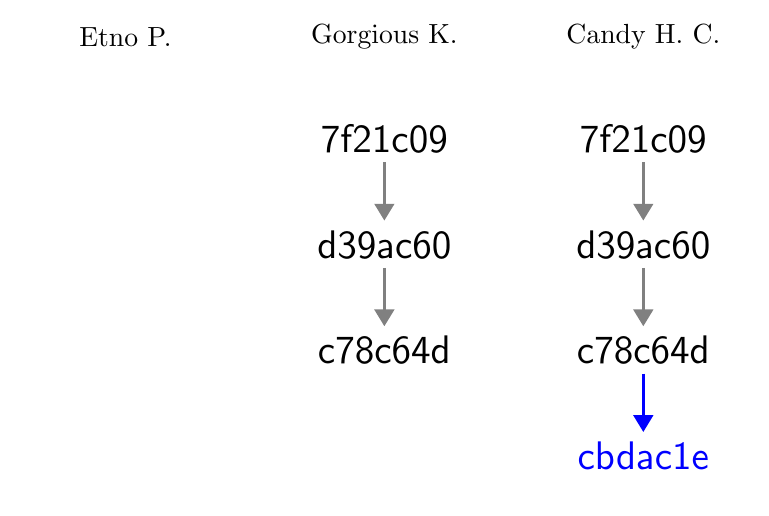
\begin{tikzpicture}
  \matrix (m)
    [
      matrix of nodes,
      nodes in empty cells,
      column sep      = 3em,
      row sep         = 5ex,
      column 1/.style = { nodes = { empty } },
      column 2/.style = { nodes = { empty } },
      column 3/.style = { nodes = { empty } },
    ]
    {
        &  &  \\
        & 7f21c09 & 7f21c09 \\  
        & d39ac60 & d39ac60 \\  
        & c78c64d & c78c64d \\  
        &  & |[high]| cbdac1e \\  
    };
    \node[fit=(m-1-1)(m-1-1)]{Etno P.};
    \node[fit=(m-1-2)(m-1-2)]{Gorgious K.};
    \node[fit=(m-1-3)(m-1-3)]{Candy H. C.};
  
    \foreach \i/\j in {2/3, 3/4} {
      \draw [arrow] (m-\i-2) -- (m-\j-2);
      \draw [arrow] (m-\i-3) -- (m-\j-3);
    }
    \draw [harrow] (m-4-3) -- (m-5-3);
\end{tikzpicture}

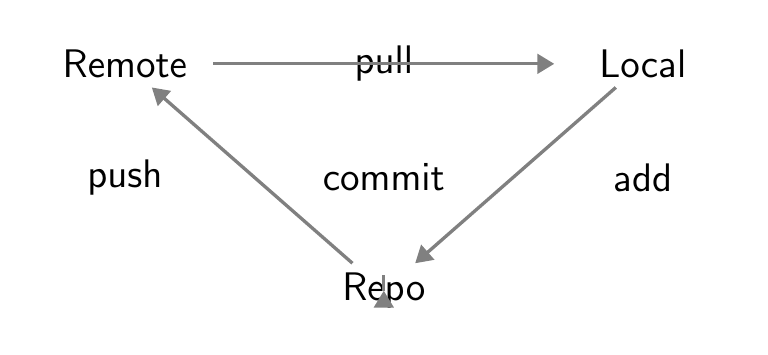
\begin{tikzpicture}
  \matrix (m)
    [
      matrix of nodes,
      nodes in empty cells,
      column sep      = 3em,
      row sep         = 5ex,
      column 1/.style = { nodes = { empty } },
      column 2/.style = { nodes = { empty } },
      column 3/.style = { nodes = { empty } },
    ]
    {
        Remote & pull & Local \\
        push & commit & add \\  
        & Repo & \\  
    };
  
    \draw [arrow] (m-1-1) -- (m-1-3);
    \draw [arrow] (m-1-3) -- (m-3-2);
    \draw [arrow] (m-3-2) -- (m-1-1);
    \draw [arrow] (m-3-2) -- (m-3-2);
\end{tikzpicture}

\end{document}